\myslide{Subtyping}
{

  \textbf{Mit dem Subtyping Beweiswerkzeug können Subtyprelationen überprüft werden} \\[6mm]
  \begin{itemgroup}{Beispiele:}
    \item Primitive Subtyprelation \\  $\TypeSubType {\TypeIntegerType} {\TypeIntegerType} $
    \item Rekursive Subtyprelation \\  $\TypeSubType{ \TypeRecType{\TypeTypeName{t} } {\TypeArrowType
       {\TypeIntegerType }{\TypeArrowType{\TypeTypeName{t}}{\TypeTypeName{t}}}}}
       {\TypeArrowType{\TypeIntegerType}{\TypeRecType{\TypeTypeName{t}}{\TypeArrowType
       {\TypeIntegerType}{\TypeArrowType{\TypeTypeName{t}}{\TypeTypeName{t}}}}}} $
    \item Objekt Subtyprelation \\     $\TypeSubType{\TypeObjectType{\TypeRowType{{\ExprIdentifier{a}}
       \colon\ {\TypeIntegerType}\ ;\ {\ExprIdentifier{b}}\colon\  \TypeBooleanType}\ ;}} 
       {\TypeObjectType{\TypeRowType{{\ExprIdentifier{b}}\colon\ {\TypeBooleanType}\ ;\ {\ExprIdentifier{c}}
       \colon\ {\TypeArrowType{\TypeIntegerType}{\TypeIntegerType}}\ ;\ {\ExprIdentifier{a}}\colon\ {\TypeIntegerType}
       \ ;}}}$
    \end{itemgroup}
}
\myslide{Subtyping - Implementierung}
{
  \begin{itemgroup}{Probleme und Lösungen}
    \item Eingabe der Typen
    \catchword{neue GUI für Subtyping}
    \item Es dürfen nur Typen und keine Expression eingeben werden
    \catchword{Eingabe wird direkt geparst}
    \item Speichern der Dateien
    \catchword{neue Sprachen LxSUB}
    \item Für Subtype Eingaben machen die Beweiswerkzeuge für Expressions keinen Sinn
    \catchword{Ausblenden von Beweiswerkzeugen die nicht sinnvoll sind}
    \end{itemgroup}
}

\myslide{Subtyping - GUI Sourcecode}
{
  \begin{itemgroup}{Eigenschaften der GUI}
    \item Zwei Eingabefelder
    \item Zwei Outlines
    \item Einstellmöglichkeiten für Outline nur einfach
    \item Bei Ausschneiden, Einfügen, Kopieren, Wiederholen und Rückgängig machen wird die Aktion auf dem momentan
    ausgewählten Eingabefeld ausgeführt.
    \end{itemgroup}
}

\myslide{Subtyping - GUI Sourcecode}
{
  \begin{center}
    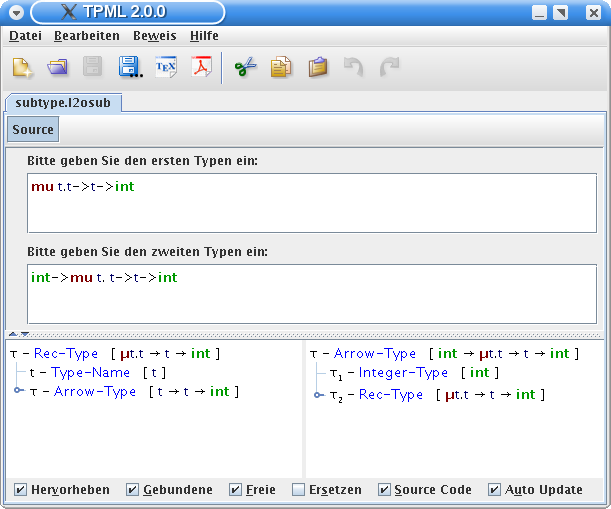
\includegraphics[height=14cm]{images/subtype.png}
  \end{center}
}